\section{Speed Estimation}\label{approach}
%Estimating User Mobility Speeds with Coarse Data Records

In this section, we systematically describe our methodology for estimating user mobility speed using coarse-grained tower communication records and timestamps.

\subsection{Methodology Overview}

Our methods consist of multiple steps, where we first decompose traces of each user into segments to zoom into intra-cell speed estimation. Next, we estimate the distance and the travel time for each segment, where we employ a distance lower bound to filter out low-confidence estimates. In practice, such estimates are usually too noisy to be meaningful or reliable. Finally, we demonstrate how to compensate for speed estimation errors. \autoref{fig:system_overview} shows the structural overview of this methodology. The raw data parser on one end of this figure gathers data access records by users and sorts records of each user by time. On the other end, a list of tower locations from the mobile data access traces is extracted. Note that the system assigns a list for each city during processing steps.

After we have parsed raw traces, we next process them in different steps in parallel. In one of the next steps, we analyze traces of each user and generate pass-boundary events (PBEs) with the timestamp and location estimates of each record. Based on these events, we can estimate intra-cell travel distances and time accordingly.

In the second sequence of steps, we process the tower list for each city, by generating a Voronoi diagram based on tower coordinates. Here, Voronoi diagrams are used to simulate the tower coverage map, based on which we calculate all intra-cell boundary-to-boundary distance lower bounds. We keep such bounds in a separate list for lookup needs.

Finally, at the end of both processing sequences, we aggregate their results to estimate each user's speed distributions. We observe that for some segments, we do not have sufficient location information to accurately estimate a particular user's speed. Under such scenarios, we develop a compensation step where we try to infer the most likely speed based on speed distributions of this user in adjacent segments. The assumption is that one user will not change speed too much in short distances. We next discuss each component in more details in the following sections.

\subsection{Pass-Boundary Events}

%As our dataset is coarse-grained, we only have location information of the towers with which a user communicates. 
As a user could be anywhere inside the tower's coverage area, we need to infer their speeds by exploiting multiple coverage areas. To this end, we first decompose the trace into segments, which we call ``pass-boundary events'' (PBE).

\begin{figure}[h]
    \centering
    %\vspace{-0.1in}
    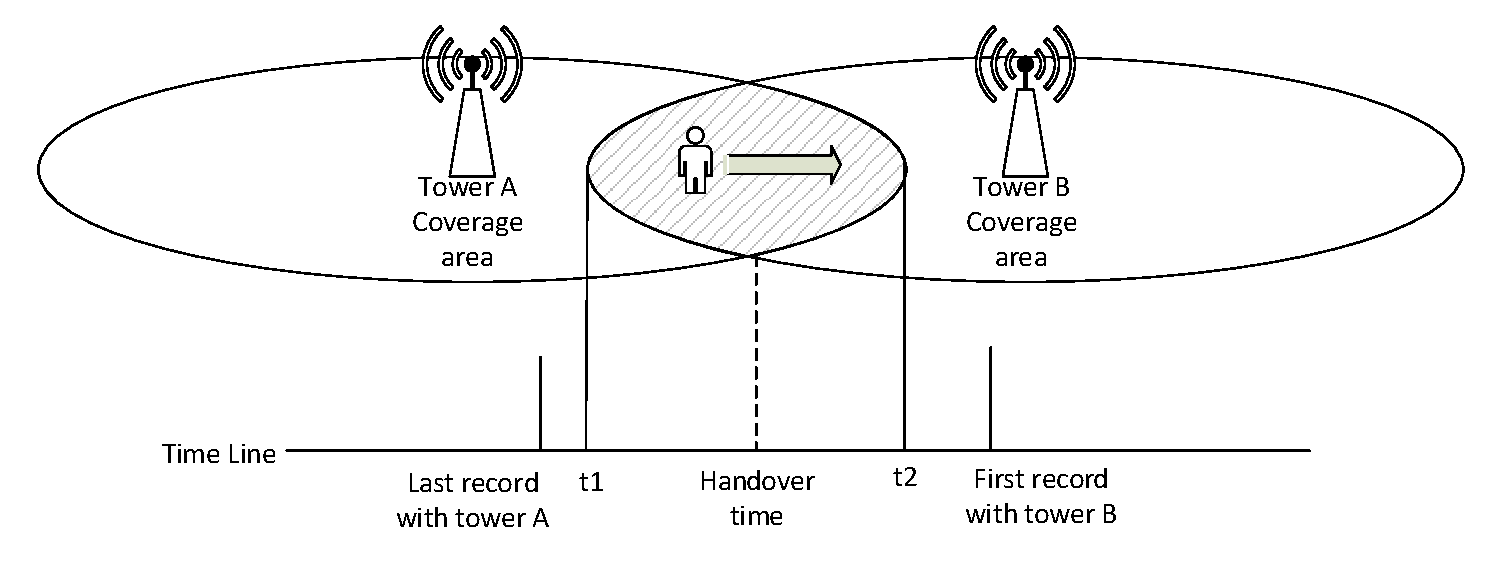
\includegraphics[width=\linewidth]{./figures/passing_boundary.pdf}
    \vspace{-0.3in}
    \caption{A pass-boundary event.}
    \label{fig:pass_bound}
\end{figure}


Formally, a PBE is defined as when a user moving from one tower's coverage cell into an adjacent tower's coverage cell. There are two properties related to a PBE: first, each PBE has a boundary area, which is the overlapping coverage area of two towers; second, each PBE is associated with a time period of the user spent on crossing the boundary area. For example, in \autoref{fig:pass_bound}, the PBE event is associated with a boundary as the shadowed area, while its associated time period is $(t_1, t_2)$ for entering and leaving this shadow area.

We now describe the algorithm on extracting PBEs from the mobile data access traces. For arbitrary two consecutive records $r_i$ and $r_j$ of a user with $l_i$ and $l_j$ as their location estimates respectively, if $l_i \neq l_j$, we define a PBE, denoted by $P_{i, j}$ as follows:
\[
P_{i,j} = (r_i, r_j)
\]
We denote the boundary of $P_{i, j}$, which is the overlapped area, as $(l_i, l_j)$. We use $({t_i}^{last}, {t_j}^{first})$ as an estimate of the time period of entering and leaving $P_{i, j}$, where ${t_i}^{last}$ is the last record timestamp in $l_i$, and ${t_j}^{first}$ is the first record timestamp in $l_j$. The length of the time period of $P_{i, j}$ is bounded by ${t_j}^{first} - {t_i}^{last}$.
Once PBEs are defined, we use them as reference points to decompose mobile data records of each user into segments.

\begin{algorithm}
 \KwData{$Trace$: mobile data trace arranged by users $u$ with record entries $e$ sorted by time. Each $e$ has location estimate $l_e$ and timestamp $t_e$}
 \KwResult{$R$: segments $r$ arranged by user and time.}
 \For{each $u$ in $Trace$}{
	 $l_c \gets \emptyset$,
	 $r \gets \emptyset$,
	 $e_{lastend} \gets \emptyset$,
	 $e_{start} \gets \emptyset$,
	 $e_{end} \gets \emptyset$ \;
	 \For{each $e$ in $Trace[u]$}{
		 \If{$l_c \neq \emptyset$ and $l_c \neq l_e$}{
			 $l_r \gets (l_{e_{lastend}}, l_c, l_e)$,
			 $t_r \gets (t_{e_{start}}, t{e_{end}})$ \;
			 append $r$ to $R[u]$ \;
		 }
		 \If{$l_c = \emptyset$ or $l_c \neq l_e$}{
			 $e_{lastend} \gets e_{end}$,
			 $l_c \gets l_e$,
			 $e_{start} \gets e$
		 }
		 $e_{end} \gets e$ \;
	 }
	 $l_r \gets (l_{e_{lastend}}, l_c, l_e)$,
	 $t_r \gets (t_{e_{start}}, t{e_{end}})$ \;
	 append $r$ to $R[u]$ \;
 }
 \Return{$R$}
 \caption{Data segmentation}\label{alg:Data_segmentation}
\end{algorithm}

The detailed segmentation algorithm is shown in \autoref{alg:Data_segmentation}. Specifically, the decomposition works as follows: we first generate the PBEs for each user, and then we consider all records of a user between two consecutive PBEs as one single stretch of \emph{continuous stay} as such records should be communicating with the same tower. Therefore, they should share the same location estimate. Since we do not have observations on the intra-cell trajectories of user mobility, we consider the user to have the single constant speed for each stretch within a cell, i.e., between two PBE events. To estimate this speed, we use two consecutive PBEs. 
Note, however, that as the first and the last stretches of records only have one PBE each, they will not have speed estimates.

\subsection{Distance and Time Estimation}

We next describe how we estimate the speed between two PBEs. Specifically, we need to estimate the intra-cell boundary-to-boundary distance and the travel time. As the only available information for distance estimation is tower coordinates and tower visiting orders, for a segment with two PBEs $P_{i,j}$ and $P_{j,k}$, we use a straight line trajectory $l_i \rightarrow l_j \rightarrow l_k$ that passes all three tower $l_i$, $l_j$ and $l_k$ as an estimated trajectory. With the coordinates of towers, the euclidean distance between towers, $d(l_i,l_j)$ and $d(l_j,l_k)$, can be calculated. Since the boundaries are perpendicular bisectors of lines connecting towers (as we use Voronoi diagrams to represent cell coverage areas), the travel distance can be estimated by $\frac{d(l_i,l_j) + d(l_j,l_k)}{2}$. Note that if more information such as the underlying road networks are provided, the road trajectories that has the maximum likelihood to match visited tower sequences can also be used instead of the straight line trajectories.

The travel time of a segment is calculated by the time difference of two related PBEs. Since each PBE has a time interval associated with it for entering and leaving the overlapping area, we can calculate a range of possible values for travel time estimation, including both a tight bound and a relaxed bound. The former one suggests the shortest possible travel time to move through the area, while the latter one indicates the longest possible travel time. For example, for two PBEs $P_{i,j}$ and $P_{j,k}$ with a time interval of $({t_i}^{last}, {t_j}^{first})$ and $({t_j}^{last}, {t_k}^{first})$, respectively, we can easily derive the tight bound as $\Delta t_{tight} = {t_j}^{last} - {t_j}^{first}$ and the relaxed bound is $\Delta t_{loose} = {t_k}^{first} - {t_i}^{last}$.

\subsection{Distance Lower Bounds}

In this section, we introduce the concept of distance lower bounds. This is motivated by the observation that it is usually hard to accurately estimate the true distances of users using the coverage areas of given towers for all possible trajectories and represent them with a single distance estimate. To see this, we show an example in \autoref{fig:illustrate_cases}.

\begin{figure}[h]
    \centering
    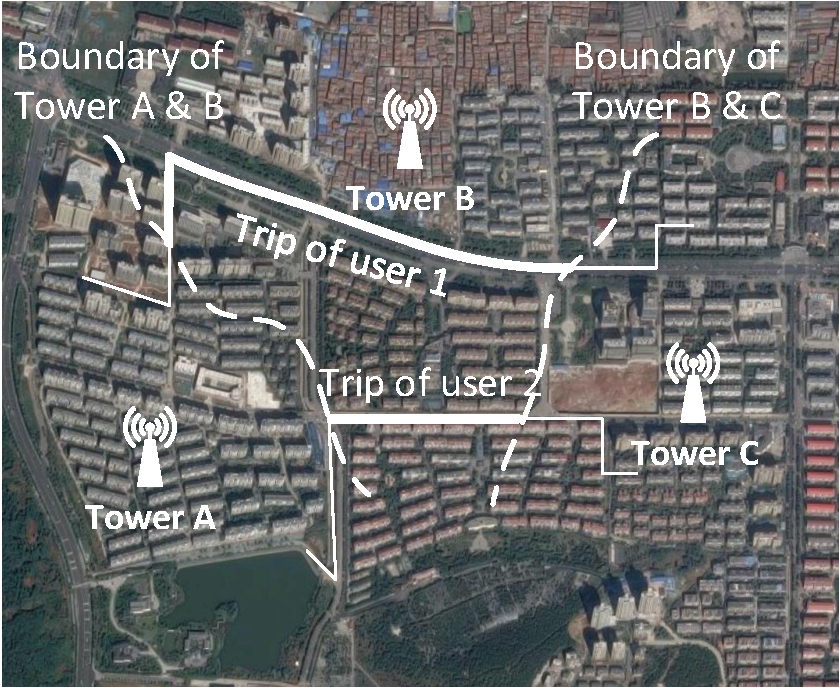
\includegraphics[width=\linewidth]{./figures/illustrate_cases.pdf}
    \vspace{-0.4in}
    \caption{Common cases where a single distance estimate would fail.}
    \label{fig:illustrate_cases}
    \vspace{-0.1in}
\end{figure}

As shown in \autoref{fig:illustrate_cases}, the area is divided into coverage areas of three towers $A$, $B$, and $C$. Solid lines represent real user trajectories while dashed lines represent the boundaries of towers. Observe that both user $1$ and user $2$ pass the three towers in the same order $A - B - C$. The real distance differences, however, are missing due to the limited location estimation accuracy of using tower locations. Therefore, in such cases, a single distance estimate will have to fail due to the wide variety of possible trajectories that can lead to the same tower visiting orders.

Faced with this challenge, our next goal is to filter out distance estimates that are not likely to occur in real world scenarios, and provide the trajectory that is most likely as the solution. The major step here is to evaluate the confidence levels of different distance estimates based on estimated trajectories and tower locations so that such confidence levels can be used as measures for evaluating differences in multiple trajectory lengths. Specifically, for two consecutive boundary events $P_{i,j}$ and $P_{j,k}$, the confidence level of a distance estimate $d_{est}$ is defined as $C_{d_{est}} = \frac{d_{lb}}{d_{est}}$, where $d_{lb}$ is the boundary-to-boundary distance lower bound, i.e., the minimum required distance to travel from the boundary of $P_{i,j}$ to the boundary of $P_{j,k}$, which serves as a conservative estimate for the shortest distance a user may travel. Intuitively, the longer an estimated distance is compared to this lower bound, the less likely it should be as it requires a more complex trajectory shape to be feasible.

\begin{figure}[h]
    \centering
    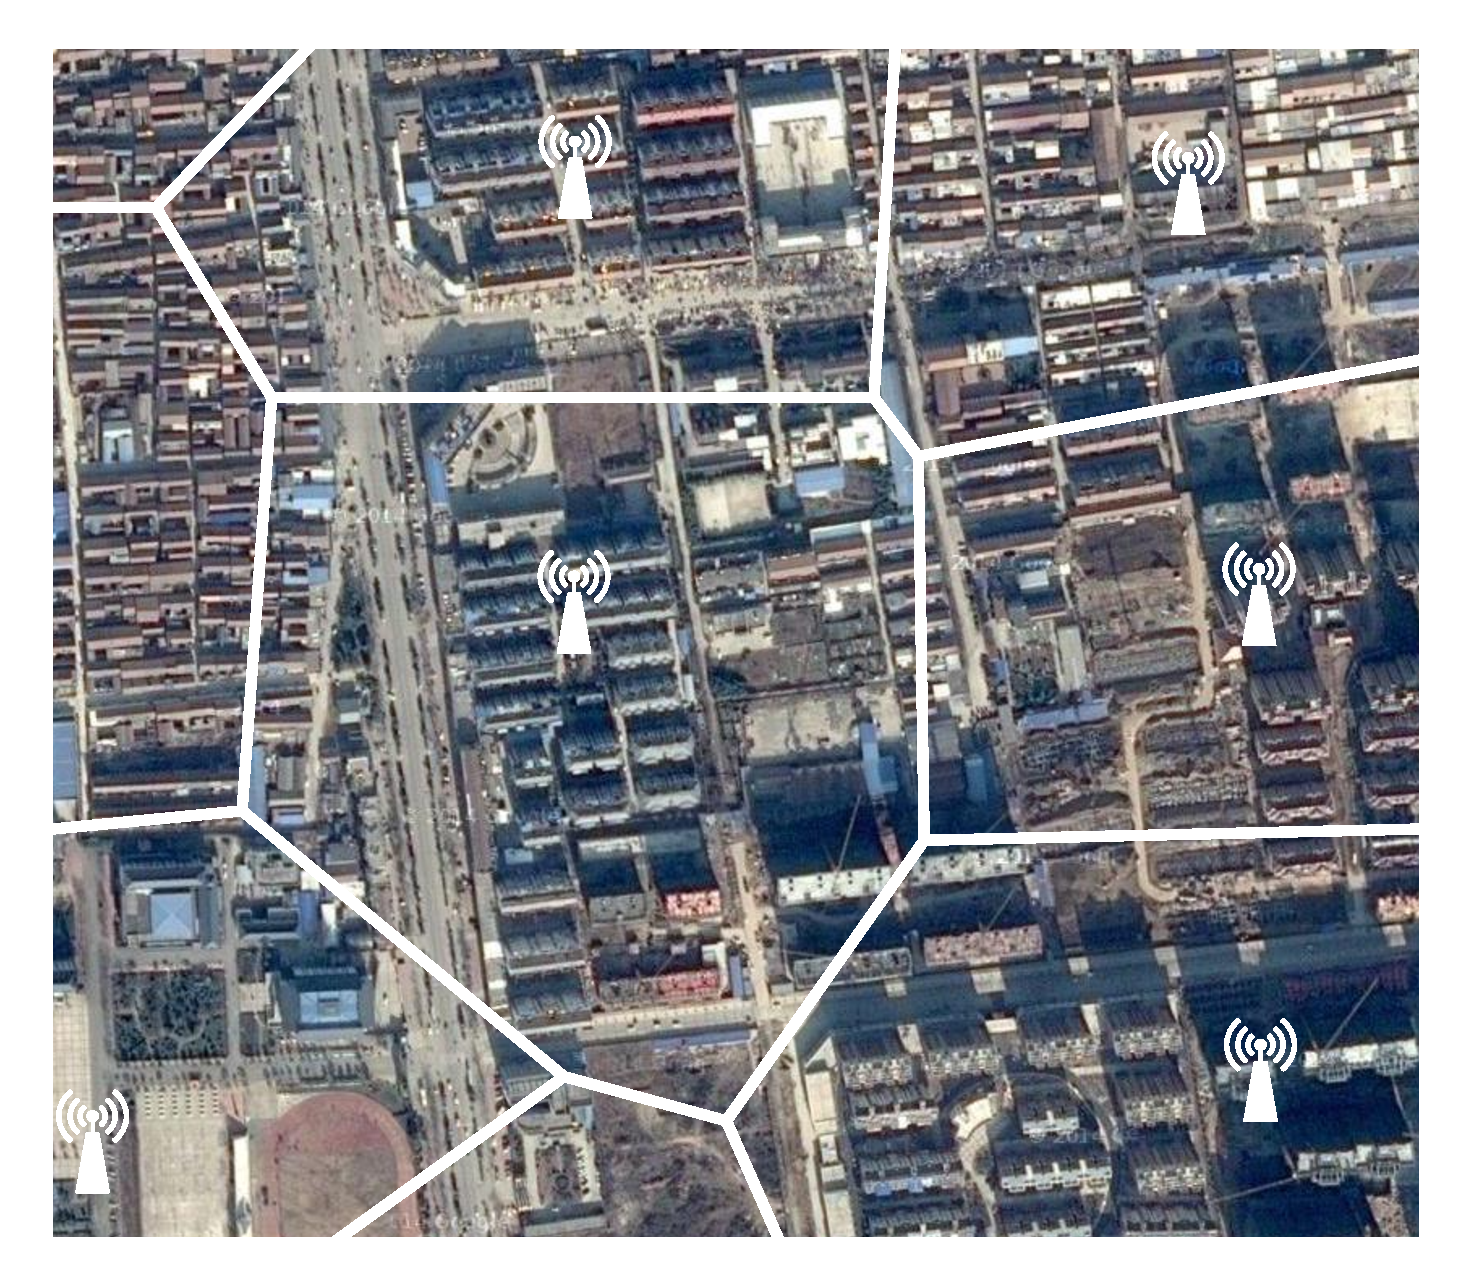
\includegraphics[width=0.9\linewidth]{./figures/voronoi_illustrate.pdf}
    \vspace{-0.1in}
    \caption{Voronoi diagram to represent communication coverage of each tower.}
		\label{fig:voronoi}
    %\vspace{-0.1in}
\end{figure}

In order to calculate the distance lower bound, 
we first simplify the tower coverage model with the Voronoi diagram. 
%the assumption that 
%cell phones only communicate with the nearest tower, 
%and towers have same transmission power. 
Then, based on the Voronoi diagram formed by towers' locations, we calculate the Voronoi cell shapes with their vertex locations. 
\autoref{fig:voronoi} shows an example of the Voronoi diagram construction with five towers. 
Each region in the Voronoi diagram represents the coverage area of one tower, while the edges in Voronoi diagrams are central focus lines of overlapping coverage area of towers (such areas are hidden in simple Voroni diagrams, but they widely exist in real-world tower communications).  
The shortest travel distance between boundaries is therefore transformed into the shortest distance between two Voronoi edges, 
and can be solved using simple geometric methods. The detailed algorithm is shown in \autoref{alg:DLB_estimation}.

\begin{algorithm}
 \SetKwComment{comment}{//}{}
 \KwData{$TC$: a list of tower coordinates.}
 \KwResult{$D_{lb}$: a list of all boundary-to-boundary distance lower bounds estimated from Voronoi diagram.}
 %\comment{project to euclidean space with equirectangular projection}
 $TL \leftarrow TC$; $P \leftarrow TL$ \;
 Build Voronoi diagram $VD$ with $P$ \;
 \For{each $edge1$ in $VD$}{
	 $pset1 \gets$ Voronoi points of $edge1$ \;
	 \For{each $edge2$ in $VD$}{
		 $pset2 \gets$ Voronoi points of $edge2$ \;
		 \If{$pset1 \cap pset2 \neq \emptyset$}{
			 $D_{lb}[(pset1, pset2)] \gets |edge1 - edge2|$\;
		 }
	 }
 }
 \Return{$R$}
 \caption{Distance lower bound estimation}\label{alg:DLB_estimation}
\end{algorithm}

%If we have an estimated distance that is much longer than the distance lower bound, then the possibility that there are trajectories of large distance differences connecting two boundaries is high. Therefore, the confidence level of using the distance estimate to represent the distance of all possible trajectories is low. On the contrary, if the estimated distance is very close to the distance lower bound, then the confidence level of estimated distance is high and the distance estimate should be able to represent the length of most trajectories between two boundaries.

\subsection{Virtual Boundaries}

A fundamental limitation of using cellphone-tower communication datasets is that records are only collected when mobile data accesses are happening. If the user is keeping silent, there is no way for us to know their locations. In such cases, if the user has traveled across multiple boundaries, we may encounter the following observation: we analyze the consecutive records for this user and find out that their $l_i$ and $l_j$  may be far away from each other and do not necessarily share a common boundary area. If $l_i$ and $l_j$ are adjacent to each other, we say to $P_{i,j}$ has a real boundary. Otherwise, we refer to it as a virtual boundary.

Different from real boundaries that are treated as an edge in the Voronoi diagram, virtual boundaries are actually distance estimates themselves as users have passed the coverage area of several towers during a PBE within a virtual boundary. Since we do not have any information regarding which towers the user has visited in between, to calculate the distance lower bound of a virtual boundary, we instead use the shortest distance of all possible boundary pairs of $l_i$ and $l_j$ as the best estimate.

We now give an example in \autoref{fig:virtual}, where we analyze two consecutive records: $r_i$ for tower $A$ and $r_j$ for tower $B$. Since tower $A$ and tower $B$ do not share physical boundaries, they only have a virtual boundary between them. To calculate their shortest distance, we calculate the distance from each boundary of tower $A$ to each boundary of tower $B$ and use the shortest one of all boundary pairs as the estimated distance. In this example, the distance between boundary $(A, C)$ and boundary $(B, N)$ is used as the distance lower bound of the virtual boundary $(A, B)$.

\begin{figure}[h]
    \centering
    \vspace{-0.1in}
    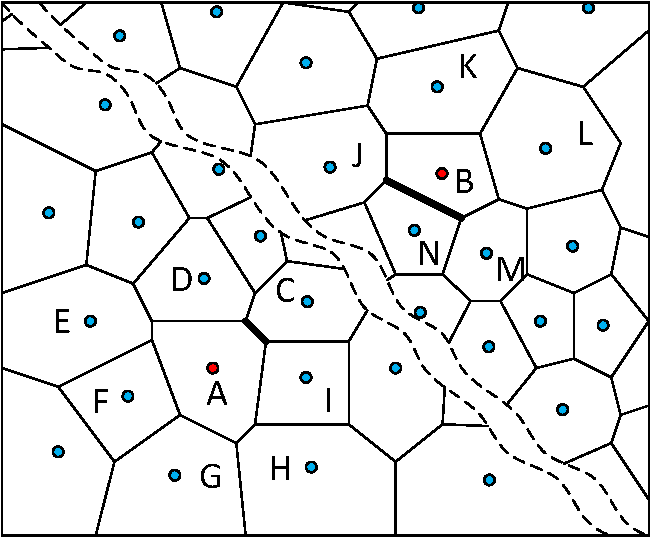
\includegraphics[width=0.9\linewidth]{./figures/virtual_boundary.pdf}
    \vspace{-0.2in}
    \caption{Dealing with virtual boundaries.}
		\label{fig:virtual}
\end{figure}

Returning to our earlier analysis, for segments that have PBEs with virtual boundaries, we merge them with adjacent segments if they exist. The distance estimate and lower bound of a segment are the sum of distance estimates and distance lower bounds of both records, and if any, the virtual boundaries between them. Note that as we calculate the sum of distance lower bounds, the resulting distance lower bound is still the minimum distance required to reach one real boundary from the other, even this requires that the trajectory should pass through virtual boundaries  between consecutively visited towers.

\subsection{Speed Estimation}

Now that we have a distance estimate $d_{est}$, a distance lower bound $d_{lb}$, and a range of possible travel time represented as $(\Delta t_{tight}, \Delta t_{loose})$ for each segment, we can infer the travel time of a segment estimated by $\Delta t_{est} = \frac{\Delta t_{tight} + \Delta t_{loose}}{2}$. We denote this by $\Delta t_{est}$. We next calculate the confidence levels for both distance estimates and travel time estimates as follows:
\begin{eqnarray}
  C_{d_{est}} &=& \frac{d_{lb}}{d_{est}} \\
  C_{\Delta t_{est}} &=& \frac{\Delta t_{est}}{\Delta t_{loose}}
\end{eqnarray}

By setting a threshold for both confidence levels, we can filter out estimates that are not accurate enough. Although we can filter out more inaccurate speed estimates with a much stricter threshold in both confidence levels, we may end up with a limited number of records that have qualified speed estimates. Finally, after setting proper threshold for confidence levels, the speed of the user can be estimated as the following:
\begin{equation}
  s_{est} = \frac{d_{est}}{\Delta t_{est}}
\end{equation}
The detail of the speed estimation algorithm is shown in \autoref{alg:speed_est}.


\begin{algorithm}
 \SetKwComment{comment}{//}{}
 \SetKwInput{KwParam}{Param}
 \KwData{$R$ from \autoref{alg:Data_segmentation} and
 %: mobile data records arranged by segments $r$;
%					$r$: A mobile data segment which has:
%					$l_{pre}, l, l{post}$: location estimates for segment before $r$, itself and segment after $r$, where $l_{pre}$ and $l_{post}$ are acquired during BPE extraction;
%					$d_{est}$:distance estimates;
%					($\Delta t_{tight}$, $\Delta t_{loose}$): travel time estimates;
          $D_{lb}$ from \autoref{alg:DLB_estimation}. %: a list of boundary-to-boundary distance lower bound estimated from Voronoi diagram.
          }
 \KwParam{$T_{C_{d}}$, $T_{C_{t}}$: confidence level threshold for distance estimates and travel time estimates.}
 \KwResult{$S$: Speed estimates for each segment.}
 \For{each $r$ in $R$}{
	 \comment{Check if $r$ has real boundary and find its distance lower bound}
	 \eIf{$((l_{pre}, l), (l, l_{post}))$ is not in $D_{lb}$}{
		 combine $r$ with next record \;
		 continue \;
	 }
	 {
		 $d_{lb} \gets D_{lb}[(l_{pre}, l), (l, l_{post})]$ \;
	 }
	 \comment{Calculate travel time estimates}
	 $\Delta t_{est} \gets \frac{\Delta t_{tight} + \Delta t_{loose}}{2}$ \;
	 \comment{Calculate confidence level}
	 $C{d_{est}} \gets \frac{d_{lb}}{d_{est}}$ ;
	 $C_{\Delta t_{est}} \gets \frac{\Delta t_{est}}{\Delta t_{loose}}$ \;
	 \comment{Estimate speed if meet threshold}
	 \If{$C{d_{est}} \geq T_{C_{d}}$ and $C_{\Delta t_{est}} \geq T_{C_{t}}$}{
		 $s_{est} \gets \frac{d_{est}}{\Delta t_{est}}$ ;
		 $S[r] \gets s_{est}$ \;
	 }
 }
 \Return{$S$}
 \caption{Speed estimation}\label{alg:speed_est}
\end{algorithm}


\subsection{Cell Oscillation and Speed Compensation}

The distance lower bounds can also help to eliminate the cell oscillation problem, i.e., when a user near boundary area randomly communicates with two or more towers in short periods, generating a sequence of false pass-boundary events. Since the user keeps passing the same boundary, the distance lower bound for such scenarios should always be $0$. Therefore, the confidence level of distance estimates will also be $0$, which means that we can detect them and filter them out.

Since segments between these false PBEs usually have very short durations due to the nature of how they are generated, we estimate the speed for such segments based on the assumption that a user's speed does not change dramatically in a very short time period. Therefore, for a segment between false PBEs, if there is a segment that happens to be very close to it and has a qualified speed estimate,  we will use its speed estimate as the speed estimate for the segment with false PBEs. Other kinds of low confident level speed estimations can also be compensated by the nearby segments with high confidence levels as long as the confidence level and time period are properly handled.

